\let\negmedspace\undefined
\let\negthickspace\undefined
\documentclass[journal]{IEEEtran}
\usepackage[a4paper, margin=10mm, onecolumn]{geometry}
%\usepackage{lmodern} % Ensure lmodern is loaded for pdflatex
\usepackage{tfrupee} % Include tfrupee package

\setlength{\headheight}{1cm} % Set the height of the header box
\setlength{\headsep}{0mm}  % Set the distance between the header box and the top of the text

\usepackage{gvv-book}
\usepackage{gvv}
\usepackage{cite}
\usepackage{amsmath,amssymb,amsfonts,amsthm}
\usepackage{algorithmic}
\usepackage{graphicx}
\usepackage{float}
\usepackage{textcomp}
\usepackage{xcolor}
\usepackage{txfonts}
\usepackage{listings}
\usepackage{enumitem}
\usepackage{mathtools}
\usepackage{gensymb}
\usepackage{comment}
\usepackage[breaklinks=true]{hyperref}
\usepackage{tkz-euclide} 
\usepackage{listings}
% \usepackage{gvv}                                        
\def\inputGnumericTable{}                                 
\usepackage[latin1]{inputenc}                                
\usepackage{color}                                            
\usepackage{array}                                            
\usepackage{longtable}                                       
\usepackage{calc}                                             
\usepackage{multirow}                                         
\usepackage{hhline}                                           
\usepackage{ifthen}                                           
\usepackage{lscape}
\usepackage{tikz}
\usetikzlibrary{patterns}

\begin{document}

\bibliographystyle{IEEEtran}
\vspace{3cm}

\title{10.7.7}
\author{ee25btech11063-vejith}

\maketitle
% \maketitle
% \newpage
% \bigskip
{\let\newpage\relax\maketitle}
\renewcommand{\thefigure}{\theenumi}
\renewcommand{\thetable}{\theenumi}
\setlength{\intextsep}{10pt} % Space between text and floats
\textbf{Question}\\
The slope of the line touching both the parabolas y$^2$ = 4x and x$^2$ = -32y is\\
\textbf{Solution}:\\
The equation of a parabola in Matrix form is
\begin{align}
\vec{x}^\top\vec{V}\vec{x} + 2\vec{u}^\top\vec{x} + f = 0
\end{align}
For y$^2$=4x
\begin{align}
    \vec{V_1}=\begin{pmatrix}
        0 & 0\\
        0 & 1
    \end{pmatrix}\\
    \vec{u_1}=-2\vec{e_1}=\myvec{-2\\0}\\
    f_1=0\\
    \implies \vec{x}^\top \begin{pmatrix}
        0 & 0\\
        0 &1
    \end{pmatrix}\vec{x} +2\myvec{-2\\0}\vec{x}=0
\end{align}
For x$^2$=-32y
\begin{align}
    \vec{V_2}=\begin{pmatrix}
        1 & 0\\
        0 & 0
    \end{pmatrix}\\
    \vec{u_2}= 16\vec{e_2}=\myvec{0\\16}\\
    f_2=0\\
    \implies \vec{x}^\top \begin{pmatrix}
        1 & 0\\
        0 & 0
    \end{pmatrix}\vec{x} +2\myvec{0\\16}\vec{x}=0
\end{align}
a line $\vec{x}$=$\vec{h}$ +k$\vec{m}$ touches (1) if
\begin{align}
    \vec{m}^\top \brak{\vec{V}\vec{q}+\vec{u}}=0 
    \brak{\text{where $\vec{q}$ is the point of contact}}
\end{align}
\begin{align}
     \vec{m}^\top \brak{\vec{V_1}\vec{q_1}+\vec{u_1}}=0\\
      \vec{m}^\top \brak{\vec{V_2}\vec{q_2}+\vec{u_2}}=0 
\end{align}
let 
\begin{align}
    \vec{q_2}-\vec{q_1} = c\vec{m}
     \brak{\text{for some scalar }c}
\end{align}
substitute (13) in (12)
\begin{align}
    \implies  \vec{m}^\top \brak{\vec{V_2}\brak{\vec{q_1}+c\vec{m}} + \vec{u_2}}=0\\
    \implies \vec{m}^\top\vec{V_2}\vec{q_1}+ \vec{m}^\top\vec{V_2}c\vec{m} + \vec{m}^\top\vec{u_2}=0\\
    \implies \brak{1 \hspace{0.5cm} m}\begin{pmatrix}
        1 & 0\\
        0 & 0
    \end{pmatrix}\vec{q_1}+ \brak{1 \hspace{0.5cm} m}\begin{pmatrix}
        1 & 0\\
        0 & 0
    \end{pmatrix} \myvec{c\\cm} + \brak{1 \hspace{0.5cm} m} \myvec{0\\16}=0\\
  \implies  \brak{1 \hspace{0.5cm} 0}\vec{q_1}+ \brak{1 \hspace{0.5cm} 0} \myvec{c\\cm} +16m =0\\
  \implies \brak{1 \hspace{0.5cm} 0}\vec{q_1} =-c-16m
\end{align}
on expanding (11)
\begin{align}
    \implies \vec{m}^\top\vec{V_1}\vec{q_1}+  \vec{m}^\top\vec{u_1}=0\\
    \implies  \brak{1 \hspace{0.5cm} m}\begin{pmatrix}
        0 & 0\\
        0 & 1
    \end{pmatrix}\vec{q_1}+  \brak{1 \hspace{0.5cm} m} \myvec{-2\\0}=0\\
    \implies \brak{0 \hspace{0.5cm} m}\vec{q_1}=2
\end{align}\\ \\ \\ \\ 
Equations (18) and (21) can be written  as
\begin{align}
    \begin{pmatrix}
        1 & 0\\
        0 & m
    \end{pmatrix} \vec{q_1}=\myvec{-c-16m\\2}
\end{align}
The augmented matrix can be written as
\begin{align}
      \implies \left(\begin{array}{cc|c}
        1 & 0 & -c-16m \\
        0 & m & 2 
\end{array}\right)\\
\implies \vec{q_1}=\myvec{-c-16m\\ \frac{2}{m}}
\end{align}
From (13)
\begin{align}
\vec{q_2}=\vec{q_1} + c\vec{m}\\
  \implies  \vec{q_2}=\myvec{-16m\\ \frac{2}{m}+cm}
\end{align}
substitute $\vec{q_1}$ in (5)
\begin{align}
    \implies \frac{1}{{m}^2} + 16m=-c
\end{align}
substitute $\vec{q_2}$ in (9)
\begin{align}
   \implies  8m^2 + \frac{2}{m}=-cm
\end{align}
on solving (27) and (28) we get 
\begin{align}
    m=\frac{1}{2}\\
    \implies \vec{m}=\myvec{1\\ \frac{1}{2}}
\end{align}
$\implies$ slope of the line touching both the parabolas =$\frac{1}{2}$
\begin{figure}[H]
    \centering
    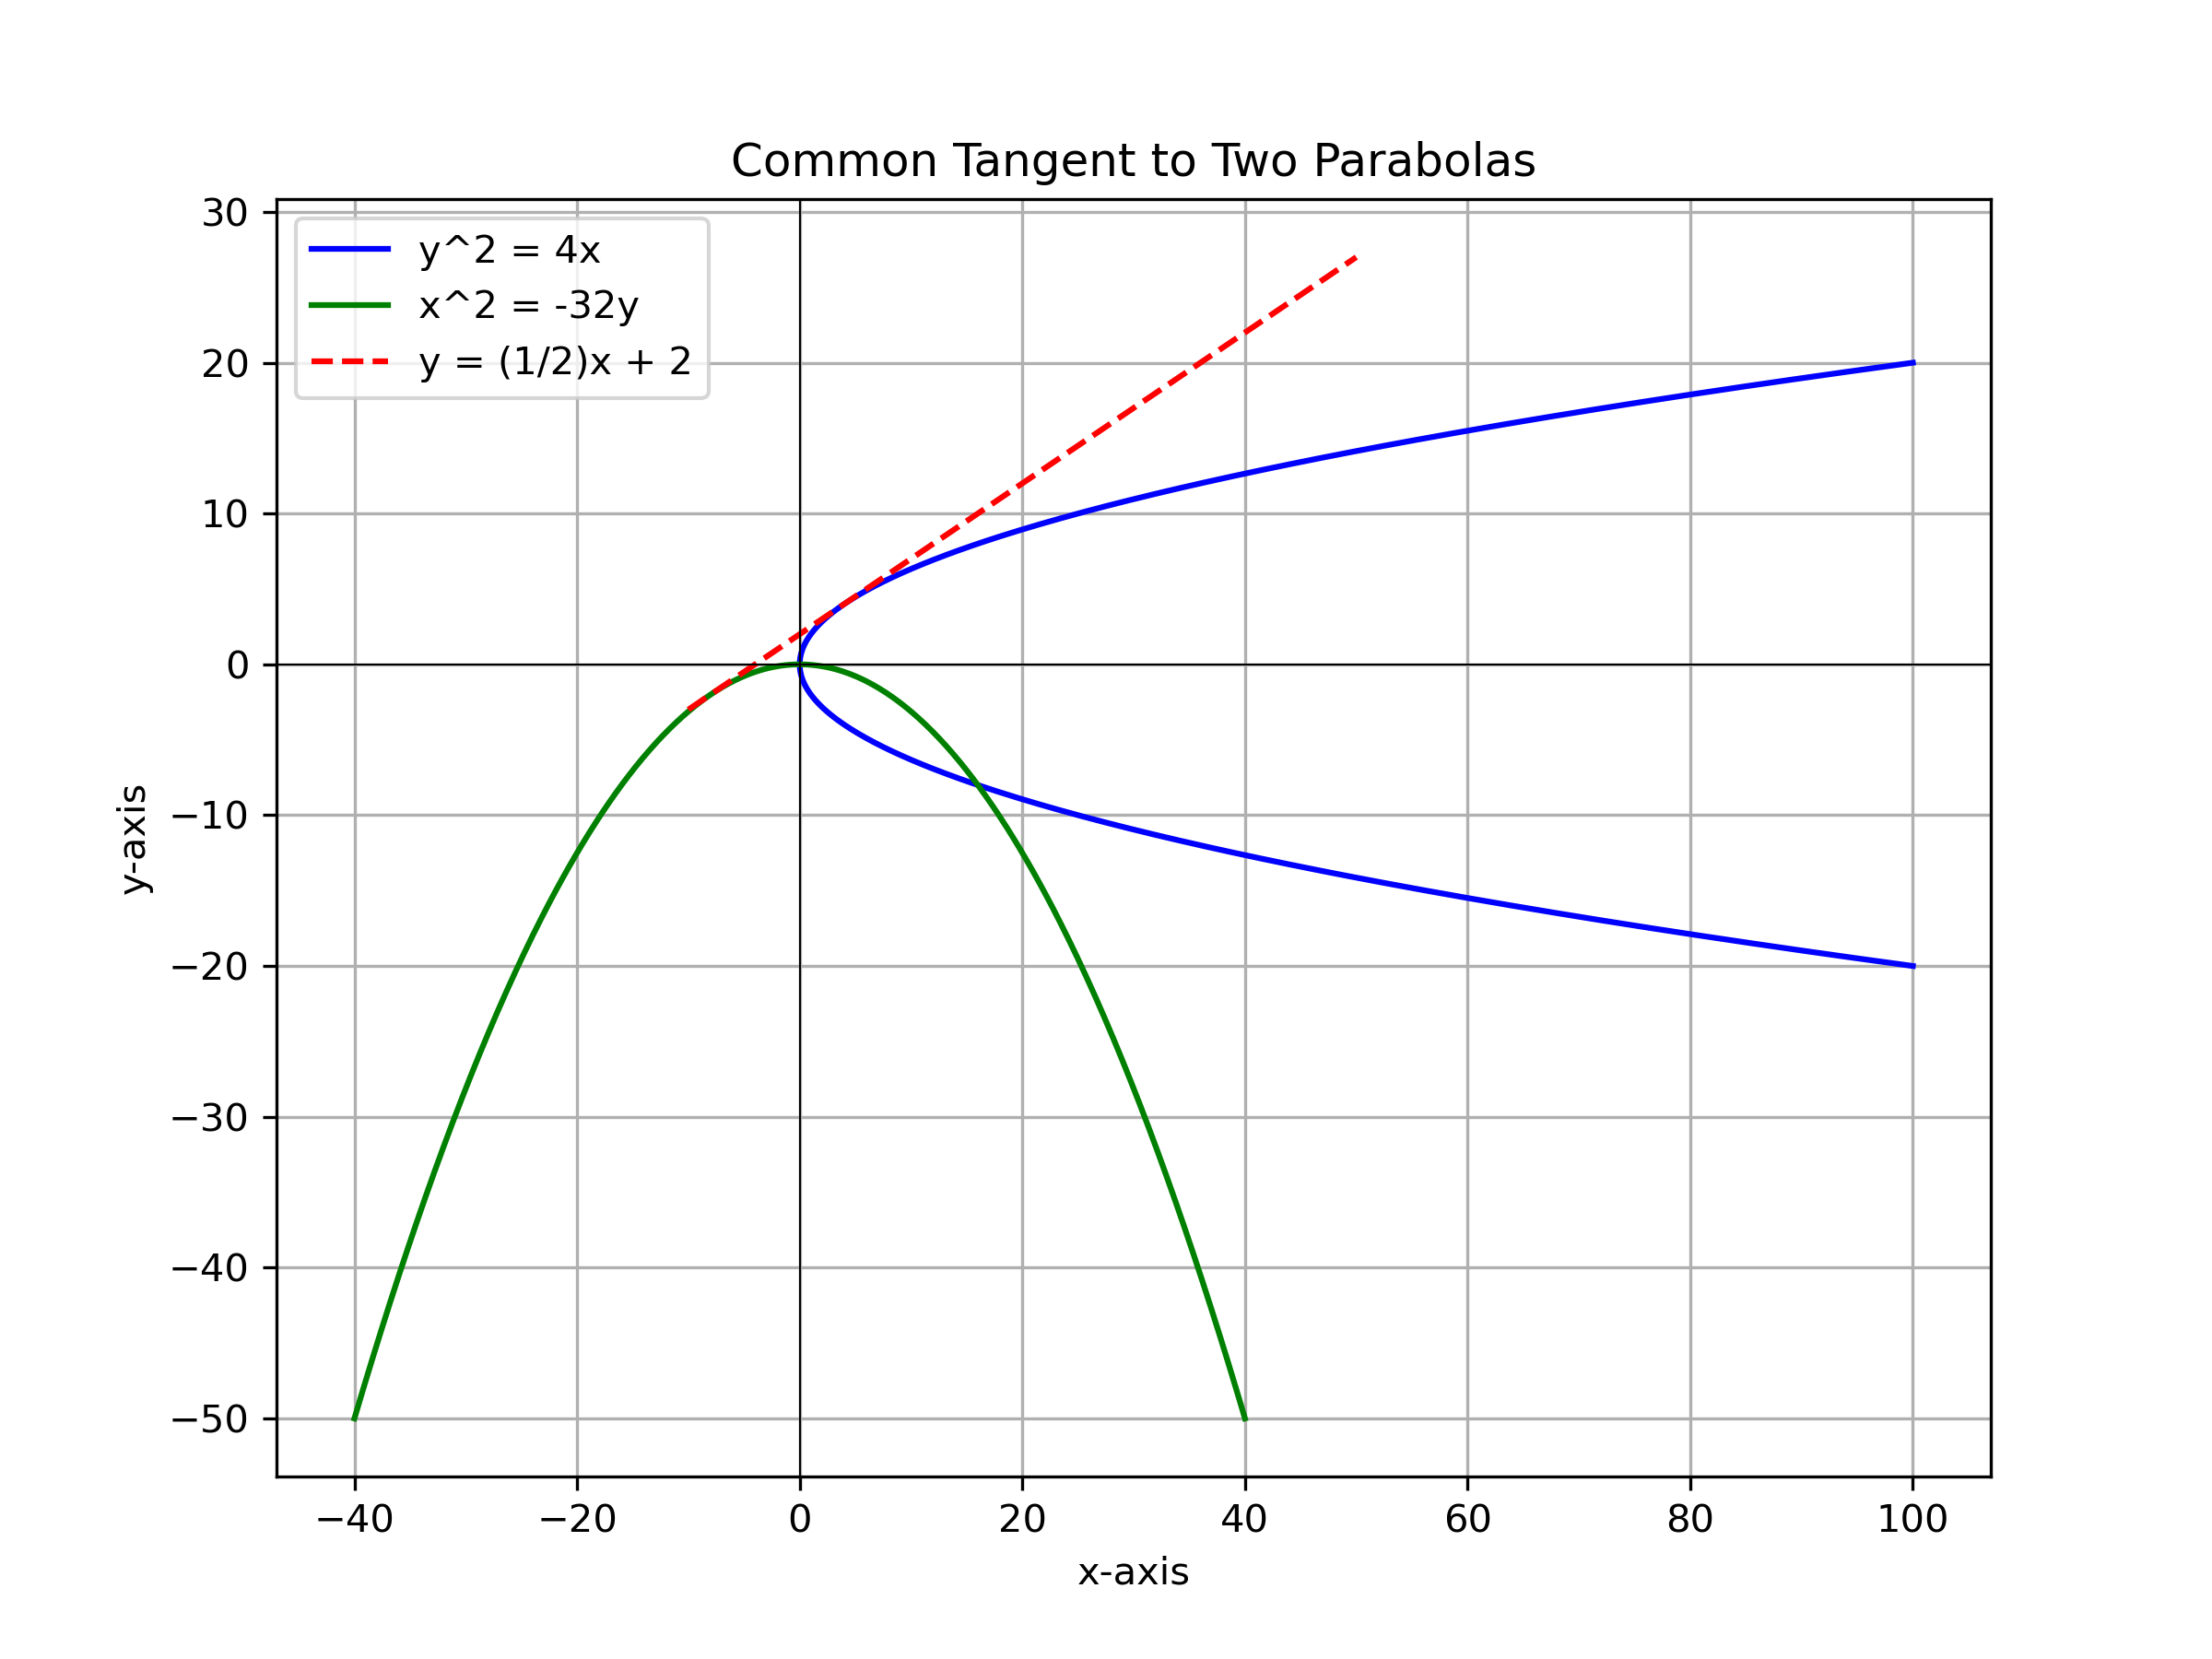
\includegraphics[width=0.8\columnwidth]{figs/01.png}
    \caption{}
    \label{fig:placeholder}
\end{figure}
\end{document}
